\documentclass[10pt]{article}
\usepackage[margin=0.8in]{geometry}
\usepackage{amsmath,booktabs,graphicx,hyperref}
\usepackage[T1]{fontenc}
\title{Learning Stochastic Image Transformations:\\Synthetic Static, Generalization, and Reversible Transport}
\author{Samuel Cavazos}
\date{October 2026}
\newcommand{\ResultStage}{Frozen test evaluation}

\begin{document}
\maketitle
\begin{abstract}
We compare independently learned image transformations with networks possessing
an explicit inverse, using 809 Pok\'emon sprites and synthetic uniform static.
The experiments distinguish recovery guaranteed by architecture from learning a
prescribed stochastic transformation. We study discrete modular noise and a
Gaussian diffusion endpoint, explicitly accounting for conditioning information
and serialized payloads. Results are labeled \emph{\ResultStage}.
This study concerns generalization and numerical transport, not cryptographic
security. Uniform static is evaluated as a training distribution, not assumed to
cover the distribution of structured images.
Across 35 short training configurations, validation selected a 44,296-parameter
Gaussian coupling model trained on sprites alone. Its held-out forward-plus-reverse
normalized mean absolute error was 0.04924, compared with 0.05155 for equal mixed
training and 0.12187 for static-only training. Thus uniform static did not improve
target learning under the tested fixed update budget. Retained byte coupling
models achieved exact serialized self-round trips across all evaluated test
domains, although agreement with the prescribed byte transformation remained
imperfect.
\end{abstract}

\section{Motivation and prior experiment}
The earlier implementation trained and evaluated on the same 809 images,
preserved alpha masks, and used a 1,000-step Gaussian schedule with signal
coefficient approximately $5.07\times10^{-12}$ before clipping and 8-bit
quantization. These conditions cannot establish general recovery of unseen RGB
content. We retain that process as a diagnostic and evaluate a silhouette-only
nearest-training-mask retrieval baseline. This baseline quantifies a shortcut;
it is not a reconstruction model trained on the test images.
\IfFileExists{generated/old-process.pdf}{
\begin{figure}[ht]
\centering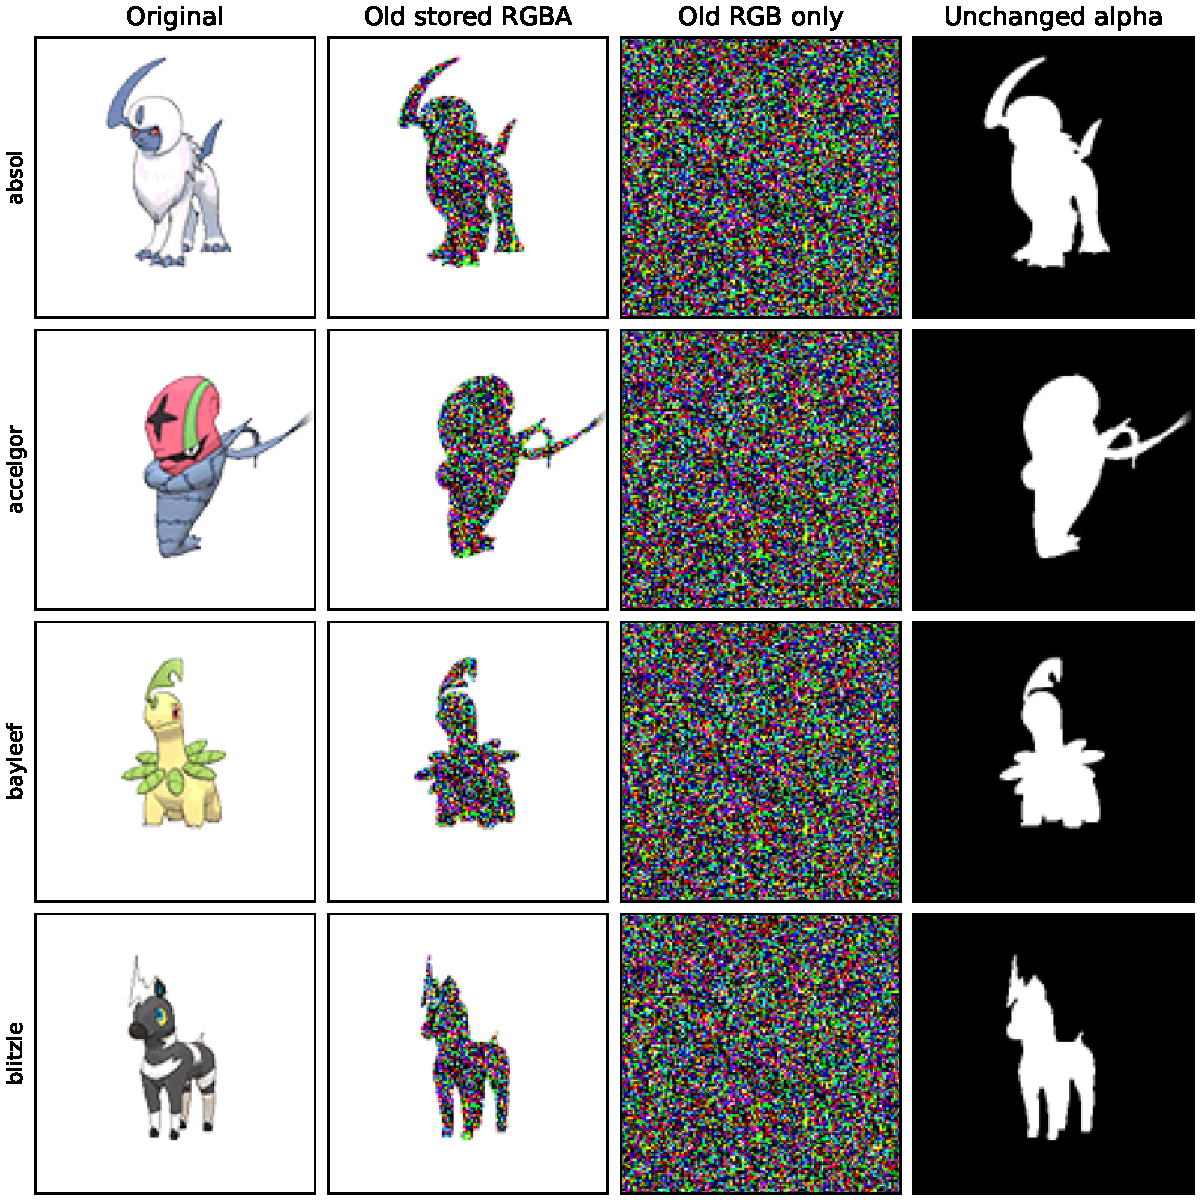
\includegraphics[width=0.72\linewidth]{generated/old-process.pdf}
\caption{The first four validation images in manifest order. Under the old process,
the RGB fields are identical; unchanged alpha carries the distinct silhouettes.
Showing only the stored RGBA render can conceal this failure.}
\end{figure}}{}

\section{Related approaches}
Real NVP introduced tractable invertible continuous coupling transformations
\cite{realnvp}. Discrete flows and integer discrete flows provide corresponding
constructions for discrete domains \cite{discrete,idf}; continuous invertibility
alone does not guarantee recovery following quantization. Efficient restoration
architectures such as NAFNet \cite{nafnet} motivate compact convolutional
comparisons, although our baseline is a plain residual CNN, not a reproduction of
NAFNet. Adversarial neural cryptography \cite{anc} addresses a different objective,
with keys and an attacker. We do not infer confidentiality from noise appearance,
reconstruction accuracy, or invertibility.

\section{Methods}
For byte tensors, the teacher is $y=(x+n)\bmod256$, with independent uniform
integer noise and inverse $x=(y-n)\bmod256$. Repeated independent modular additions
collapse into one cumulative field, so we do not pretend that increasing the
number of such steps increases expressive power. For normalized floating-point
tensors the teacher is $y=ax+n$, $a=0.5$, with
$n\sim\mathcal N(0,1-a^2)$. This is exactly the endpoint distribution of 16
Gaussian updates with $\beta=1-a^{2/16}$. The inverse is $(y-n)/a$.
Both learner directions receive the realized noise field. The analytic inverse
requires no training; learned models are studied as controlled approximation
experiments, not as more efficient substitutes for this elementary arithmetic.
Reported conditioning sizes count the full field. A compact seeded alternative
would additionally require the generator version and stream position; the
eight-byte seed field alone is not a complete transport specification.

The independent model pair consists of six residual blocks per direction with
32 channels and no downsampling or batch normalization. Byte outputs use four
256-category heads; float outputs use four regression channels. Coupling models
use four alternating half-channel updates, each conditioned on the unchanged half
and the full noise field through a small convolutional network. Integer shifts
use straight-through rounding for training and hard rounded values for inference.
The Gaussian model uses fixed coupling scales whose product matches the teacher's
attenuation. This is an explicit inductive bias favoring that architecture.
No spatial mixing teacher is included in this first campaign.
For a byte coupling block, writing the channel halves as $(x_A,x_B)$, we use
\begin{equation}
y_A=x_A,\qquad y_B=(x_B+Q(t_\theta(x_A,n)))\bmod256.
\end{equation}
Its inverse subtracts the identical rounded shift, recomputed from $y_A$ and $n$.
Here $Q$ rounds to the nearest integer with ties to even. The continuous block
instead uses $y_B=sx_B+t_\theta(x_A,n)$ with nonzero fixed $s$, inverted by
subtraction and division. Blocks are inverted in reverse order. Thus invertibility
holds independently of whether the parameters match the prescribed teacher,
subject to reproducing the numerical conditioner outputs.

Byte training uses cross entropy for independent maps and circular byte distance
for coupling maps; Gaussian training uses mean squared error. An exploratory
byte follow-up, motivated by poor endpoint learning in the initial trials, keeps
the coupling architecture unchanged and adds intermediate teacher supervision.
For each channel half, integer shifts $\lfloor n/2\rfloor$ and
$n-\lfloor n/2\rfloor$ sum to the teacher field. An auxiliary mean squared error
on shifts divided by 128 is averaged across layers and added to each direction's
loss. Intermediate inputs are teacher-forced. This intervention exposes additional
teacher information and is not an architecture-only comparison. AdamW uses learning
rate $3\times10^{-4}$, weight decay $10^{-5}$ and gradient clipping at 1.
Effective batch size is 16. Discrete coupling evaluation uses FP32 without TF32;
integer recovery depends on reproducing the same rounded conditioner outputs.
Cross-device or cross-library bitwise compatibility is not established here.

\section{Experimental protocol}
All images retain native $120\times120$ resolution. Alpha is transformed rather
than exposed as a silhouette. Approximately 80/10/10 percent of images are split
before transformation, grouping identical pixels, named variants, and available
CSV evolution links. The supplied links are incomplete, so this is not a complete
evolutionary-family holdout. Synthetic samples use independent uniform bytes in
all four channels. Training regimes are sprite only, static only, and equal mixed
batches. Evaluation also includes separate static samples and structured probes.
The frozen manifest contains 647 training, 81 validation, and 81 test images.

One epoch is defined as 100 optimizer updates. Initial screening compares 12 configurations,
followed by three guided-training byte configurations at the same update budget,
for at most 10 epochs; promoted architectures receive at most 100 epochs for each
regime and seeds 17, 29, and 43. Hardware profiling determines a shared update cap
within each phase. Fixed-noise diagnostics use the same budget as their fresh-noise
counterparts. Validation alone determines checkpoints and promotion, averaging
over data regimes. Float round-trip errors below $10^{-6}$ are treated as tied.
The executed campaign comprises 35 trained configurations: 15 screening runs at
1,000 updates, 18 repeated runs at 2,000 updates, and two fixed-noise diagnostics
at 2,000 updates. These are 10 and 20 defined epochs, respectively.
Byte ranking first prioritizes exact full-image round trips, then forward and
reverse target-byte accuracy, and finally round-trip MAE. Gaussian ranking first
uses round-trip MAE above the tolerance, then summed forward and reverse target MAE.
The main paper track is chosen by relative validation target-error improvement
over its untrained control, with absolute errors and transport formats reported
separately; this is not a security ranking.
All retained checkpoints are hashed and frozen before test access. The same test
images are paired across conditions; seed standard deviations describe training
variation and are not population confidence intervals.
After selection, fixed- and fresh-noise-trained mixed models are cross-evaluated
on both fixed and fresh validation fields. This separates performance on a known
realization from transfer to new fields without using the test set for tuning.

\section{Results}
\subsection{Architecture and training screening}
The screening table contains single-seed validation results at 1,000 updates per
configuration. Target MAE sum combines forward and reverse teacher-endpoint errors.
The guided variant uses additional intermediate supervision; comparisons with
the original coupling loss isolate that intervention without increasing model size.
\IfFileExists{generated/screening-table.tex}{
\begin{center}\scriptsize\begin{tabular}{lllrrr}
\toprule
Track & Model & Data & Target MAE sum & Round-trip MAE & Target byte \% \\
\midrule
byte & coupling & mixed & 0.69 & 0 & 0.6 \\
byte & coupling & pokemon & 0.6912 & 0 & 0.6 \\
byte & coupling & static & 0.6893 & 0 & 0.6 \\
byte & guided & mixed & 0.4093 & 0 & 16.4 \\
byte & guided & pokemon & 0.3752 & 0 & 15.2 \\
byte & guided & static & 0.4402 & 0 & 9.3 \\
byte & pair & mixed & 0.1987 & 0.1074 & 5.0 \\
byte & pair & pokemon & 0.2021 & 0.1074 & 4.7 \\
byte & pair & static & 0.8194 & 0.4917 & 0.4 \\
gaussian & coupling & mixed & 0.08548 & 7.651e-08 & -- \\
gaussian & coupling & pokemon & 0.08173 & 7.583e-08 & -- \\
gaussian & coupling & static & 0.1428 & 7.606e-08 & -- \\
gaussian & pair & mixed & 0.123 & 0.0643 & -- \\
gaussian & pair & pokemon & 0.08151 & 0.04099 & -- \\
gaussian & pair & static & 0.6099 & 0.2545 & -- \\
\bottomrule
\end{tabular}
\end{center}}{}
\subsection{Retained approaches}
The table reports mean normalized errors, with byte errors divided by 255.
Forward error measures agreement with the teacher; reverse error uses teacher
outputs; round-trip error uses the learner's own serialized output. These are
different questions. Exact image recovery and byte accuracy, per-domain results,
untrained controls, hardware costs, and per-seed values accompany the paper as
machine-readable artifacts.
Full-image errors include alpha and background RGB values. Foreground-only RGB
errors, using the original nonzero alpha mask, are recorded separately so that
background-heavy sprites do not conceal errors in visible content.
\begin{center}\small\begin{tabular}{lllrrr}
\toprule
Track & Model & Data & Forward MAE & Reverse MAE & Round-trip MAE \\
\midrule
byte & guided & mixed & 0.01822 & 0.3421 & 0 \\
byte & guided & pokemon & 0.01661 & 0.3281 & 0 \\
byte & guided & static & 0.01915 & 0.4257 & 0 \\
gaussian & coupling & mixed & 0.01718 & 0.03437 & 7.685e-08 \\
gaussian & coupling & pokemon & 0.01641 & 0.03283 & 7.583e-08 \\
gaussian & coupling & static & 0.04153 & 0.08034 & 8.194e-08 \\
\bottomrule
\end{tabular}
\end{center}
\begin{figure}[h]
\centering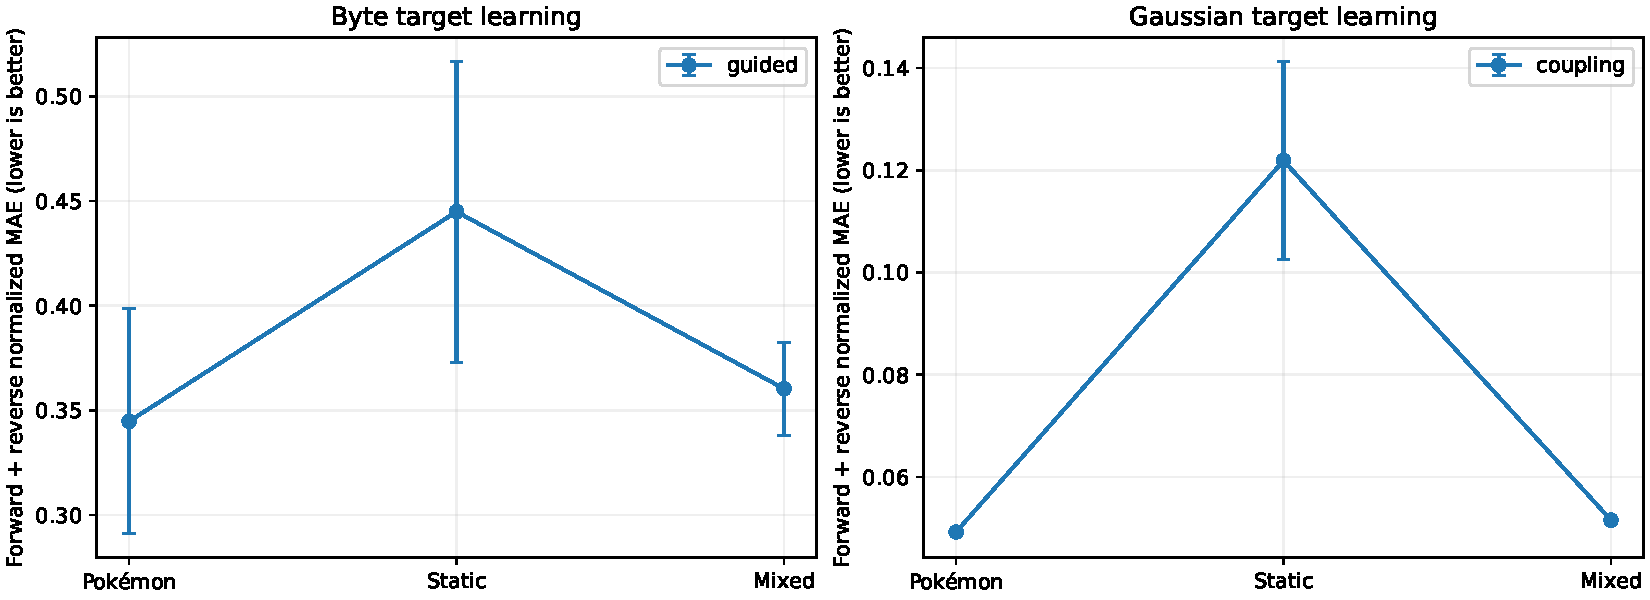
\includegraphics[width=\linewidth]{generated/comparison.pdf}
\caption{Target transformation learning across data regimes. Error bars, when
available, show sample standard deviation across three training seeds.}
\end{figure}
\IfFileExists{generated/static-transfer.pdf}{
\begin{figure}[ht]
\centering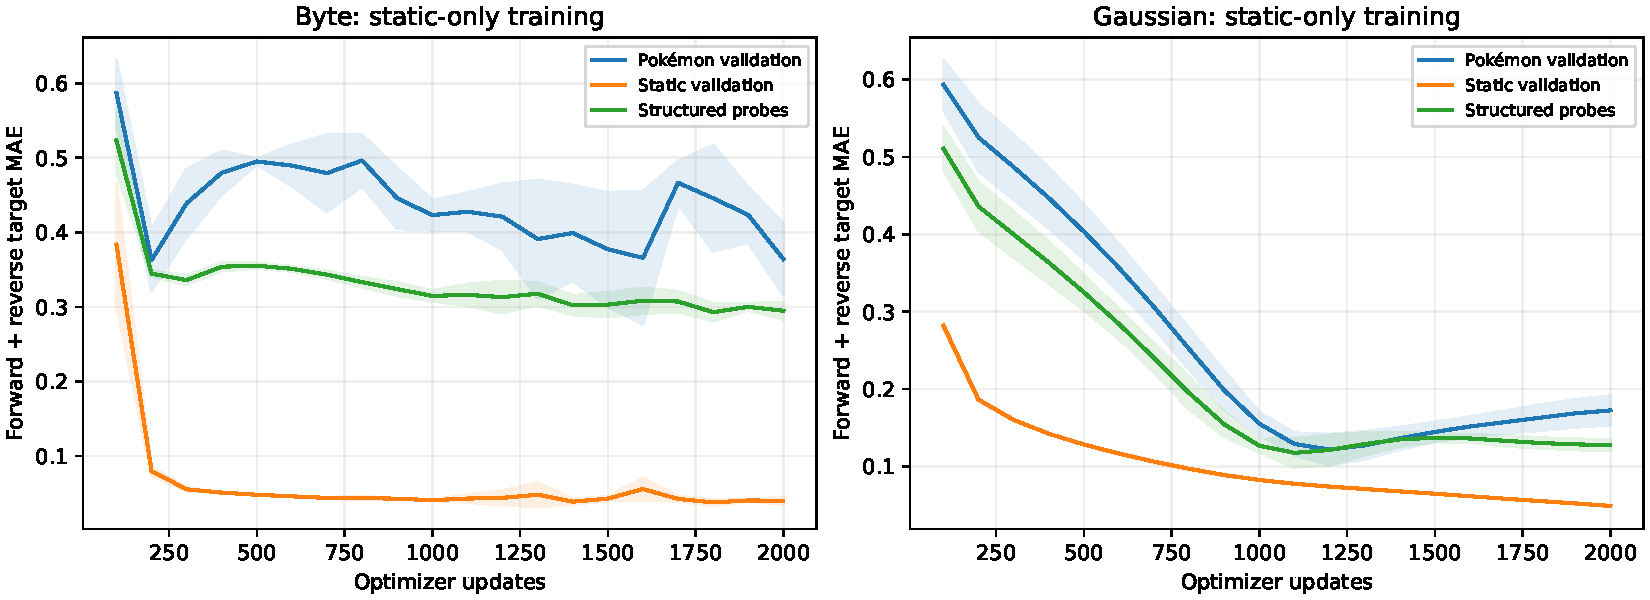
\includegraphics[width=\linewidth]{generated/static-transfer.pdf}
\caption{Validation trajectories during static-only training of retained models.
Lines average the training seeds; bands show sample standard deviation. Static,
sprite, and structured-probe errors are reported separately to expose distribution
transfer failures. These are validation trajectories, not repeated test queries.}
\end{figure}}{}
\IfFileExists{generated/conclusions.tex}{\subsection{Selection and transfer}

Validation selected the coupling architecture with pokemon training for the gaussian track as the main approach. This selection was frozen before test evaluation. Both transformation tracks and all training regimes remain reported.

For byte, the mean held-out forward-plus-reverse MAE was 0.34467 with sprite training, 0.44486 with static training, and 0.36029 with mixed training. These descriptive differences concern target learning; exact self-inversion alone is not evidence of transfer.

Byte forward-target accuracy (mean and sample standard deviation across training seeds) was pokemon: $20.88\pm0.70$\%; static: $10.59\pm0.96$\%; mixed: $19.23\pm1.01$\%. These percentages measure agreement with the prescribed teacher, not self-round-trip recovery.

For gaussian, the mean held-out forward-plus-reverse MAE was 0.049237 with sprite training, 0.12187 with static training, and 0.051555 with mixed training. These descriptive differences concern target learning; exact self-inversion alone is not evidence of transfer.

The largest Gaussian learned-round-trip error across retained test runs and domains was 1.8477e-06. This is comfortably below half an 8-bit step ($1/510$), including input float-rounding error, so rounding reconstructed values to the nearest original byte recovers the input byte grid. This is a numerical recovery property, not evidence of target learning.

\subsection{Costs and diagnostics}

Extended runs used 2000--2000 updates (20--20 defined epochs), with an effective batch size of 16. The retained coupling networks have 44,296 parameters; the independent byte and Gaussian pairs have 294,208 and 226,888 parameters respectively.

The original process yielded 1 unique RGB arrays among 81 validation images, while preserving alpha exactly. Silhouette-only nearest-training-mask retrieval achieved normalized RGB MAE 0.074125. Clipping and quantizing the gentler Gaussian endpoint to PNG produced analytic recovery MAE 0.77363; this illustrates why Gaussian results require an unclipped float payload.

\subsection{Noise realization transfer}

For byte, the fresh-noise-trained mixed model had validation target MAE sum 0.37334 on fresh fields and 0.3723 on the fixed field. The fixed-noise-trained counterpart had errors 0.36328 on fresh fields and 0.35988 on the fixed field. This single-seed diagnostic crosses training and evaluation noise conditions; it is excluded from architecture selection.

For gaussian, the fresh-noise-trained mixed model had validation target MAE sum 0.051844 on fresh fields and 0.051489 on the fixed field. The fixed-noise-trained counterpart had errors 0.059442 on fresh fields and 0.053802 on the fixed field. This single-seed diagnostic crosses training and evaluation noise conditions; it is excluded from architecture selection.
}{}

\section{Limitations and interpretation}
Exact self-inversion is a property of the coupling architecture, including before
training. It does not prove the target was learned. Both teachers are elementary
conditional transformations; results do not establish spatial, multimodal, or
unseen-transformation generalization. Static-only validation selection still uses
held-out Pok\'emon images, so the training distribution is synthetic but model
selection is not fully blind to the target domain. Small sprite data, incomplete
family metadata, differing losses and parameter counts, a single GPU, and three
training seeds constrain conclusions. Independent pairs use teacher-endpoint
supervision rather than joint cycle-consistency training; their results do not
rule out improvements from that alternative. Architecture selection is restricted
to the small candidates tested here, not a search for a globally optimal model.
At equal update budgets, the mixed regime receives half as many Pok\'emon
presentations as sprite-only training. This is a compute-budget comparison.
An exposure-matched follow-up would retain the same number of real-image
presentations and add synthetic updates, with the associated extra computation.
An unrelated GPU workload was observed during the extended trials; later wall-clock
training and inference times are descriptive shared-machine measurements, not
isolated speed benchmarks. Architecture profiling preceded that workload.
On the RTX 5070 (12 GB), profiling measured approximately 0.3--1.1 GB of peak
PyTorch tensor allocation across candidates; this excludes driver and other
process memory and is not total board usage.
Gaussian float payloads are larger than
byte tensors. Noise fields or reproducible seeds are explicit side information,
and no secrecy, authentication, resistance to chosen-plaintext attacks, or
deployment suitability is claimed. Further experiments should add spatial
coupling teachers and independently test security objectives if pursued.
To investigate the remaining distribution-transfer gap, a follow-up can compare
white static with constant-color patches and spatially correlated synthetic
textures, while retaining the same held-out evaluation discipline.

\begin{thebibliography}{9}
\bibitem{realnvp} Dinh et al. Density estimation using Real NVP. 2017.
\url{https://arxiv.org/abs/1605.08803}
\bibitem{discrete} Tran et al. Discrete Flows: Invertible Generative Models of
Discrete Data. 2019. \url{https://arxiv.org/abs/1905.10347}
\bibitem{idf} Hoogeboom et al. Integer Discrete Flows and Lossless Compression.
2019. \url{https://arxiv.org/abs/1905.07376}
\bibitem{nafnet} Chen et al. Simple Baselines for Image Restoration. 2022.
\url{https://arxiv.org/abs/2204.04676}
\bibitem{anc} Abadi and Andersen. Learning to Protect Communications with
Adversarial Neural Cryptography. 2016. \url{https://arxiv.org/abs/1610.06918}
\end{thebibliography}
\end{document}
